\documentclass[12pt,a4paper]{article}
\usepackage[margin=0.5cm]{geometry}
\usepackage{xcolor}
\usepackage{graphicx}
\usepackage{adjustbox}
\usepackage[utf8]{inputenc}
\usepackage{relsize}
\usepackage{setspace}
\linespread{0.75}
\setlength\parindent{0pt}
\begin{document}
\setlength{\fboxsep}{0pt}

\fbox{%
  % need sizes:
  % width (reduce by 0.24 cm)
  % height
  % text primary language
  % text secondary language
  % image path
  % location shortcut
  % optional: text size (default: \relscale{1} or something guessed based on existing algorithm)
  % optional: image height (otherwise half of entire size)
  \begin{minipage}[t][2.3cm][t]{17.86cm}
    \vspace{1mm}
    \setlength{\parskip}{0pt}
    \centering
    {\relscale{4.7368421052631575}
      Vorbauklemmschraube
    }

    {\relscale{5.624999999999999} Quill stem screw}

    \vspace*{-1.5\baselineskip}
    \includegraphics[height=0cm,keepaspectratio,width=17.86cm]{../../../../../Hobby/fahrrad/things-data/things/vorbauklemmschraube/image.jpg}
    \vspace*{-.8\baselineskip}
    \flushright {\tiny R-L-K-6-4}
  \end{minipage}
}

\fbox{%
  % need sizes:
  % width (reduce by 0.24 cm)
  % height
  % text primary language
  % text secondary language
  % image path
  % location shortcut
  % optional: text size (default: \relscale{1} or something guessed based on existing algorithm)
  % optional: image height (otherwise half of entire size)
  \begin{minipage}[t][3.5cm][t]{3.86cm}
    \vspace{1mm}
    \setlength{\parskip}{0pt}
    \centering
    {\relscale{1}
      Br.sattelschrauben- sicherung
    }

    {\relscale{0.9} Brake saddle screw hook}

    \vspace*{1pt}
    \includegraphics[height=1.75cm,keepaspectratio,width=3.86cm]{../../../../../Hobby/fahrrad/things-data/things/p6ryb/image.jpg}
    \vspace*{-.8\baselineskip}
    \flushright {\tiny R-L-L-14-1}
  \end{minipage}
}
\fbox{%
  % need sizes:
  % width (reduce by 0.24 cm)
  % height
  % text primary language
  % text secondary language
  % image path
  % location shortcut
  % optional: text size (default: \relscale{1} or something guessed based on existing algorithm)
  % optional: image height (otherwise half of entire size)
  \begin{minipage}[t][3.5cm][t]{4.86cm}
    \vspace{1mm}
    \setlength{\parskip}{0pt}
    \centering
    {\relscale{1.3888888888888888}
      Nabendynamo-stecker
    }

    {\relscale{1.9452651031598398} }

    \vspace*{1pt}
    \includegraphics[height=1.75cm,keepaspectratio,width=4.86cm]{../../../../../Hobby/fahrrad/things-data/things/3j8a2/image.png}
    \vspace*{-.8\baselineskip}
    \flushright {\tiny R-L-L-22-4}
  \end{minipage}
}
\fbox{%
  % need sizes:
  % width (reduce by 0.24 cm)
  % height
  % text primary language
  % text secondary language
  % image path
  % location shortcut
  % optional: text size (default: \relscale{1} or something guessed based on existing algorithm)
  % optional: image height (otherwise half of entire size)
  \begin{minipage}[t][3.5cm][t]{4.86cm}
    \vspace{1mm}
    \setlength{\parskip}{0pt}
    \centering
    {\relscale{1.3888888888888888}
      Scheibenbremsbelag
    }

    {\relscale{1.4} Disk brake pad}

    \vspace*{1pt}
    \includegraphics[height=1.6cm,keepaspectratio,width=4.86cm]{../../../../../Hobby/fahrrad/things-data/things/scheibenbremsbelag/image.jpg}
    \vspace*{-1.5\baselineskip}
    \flushright {\tiny R-L-L-12-2}
  \end{minipage}
}
\fbox{%
  % need sizes:
  % width (reduce by 0.24 cm)
  % height
  % text primary language
  % text secondary language
  % image path
  % location shortcut
  % optional: text size (default: \relscale{1} or something guessed based on existing algorithm)
  % optional: image height (otherwise half of entire size)
  \begin{minipage}[t][3.5cm][t]{4.86cm}
    \vspace{1mm}
    \setlength{\parskip}{0pt}
    \centering
    {\relscale{1.953949322370375}
      Centerlock-6-Loch-Adapter
    }

    {\relscale{1.0} Centerlock-6-bolt-adapter}

    \vspace*{1pt}
    \includegraphics[height=1.75cm,keepaspectratio,width=4.86cm]{../../../../../Hobby/fahrrad/things-data/things/centerlock_6_loch_adapter/image.jpg}
    \vspace*{-2.4\baselineskip}
    \flushright {\tiny R-L-L-11-4}
  \end{minipage}
}

\fbox{%
  % need sizes:
  % width (reduce by 0.24 cm)
  % height
  % text primary language
  % text secondary language
  % image path
  % location shortcut
  % optional: text size (default: \relscale{1} or something guessed based on existing algorithm)
  % optional: image height (otherwise half of entire size)
  \begin{minipage}[t][3.5cm][t]{4.86cm}
    \vspace{1mm}
    \setlength{\parskip}{0pt}
    \centering
    {\relscale{1.6666666666666667}
      Klicki-Teile
    }

    {\relscale{1.9452651031598398} Clicki parts}

    \vspace*{1pt}
    \includegraphics[height=1.75cm,keepaspectratio,width=4.86cm]{dummyImage.jpg}
    \vspace*{-.8\baselineskip}
    \flushright {\tiny R-L-L-22-1}
  \end{minipage}
}
\fbox{%
  % need sizes:
  % width (reduce by 0.24 cm)
  % height
  % text primary language
  % text secondary language
  % image path
  % location shortcut
  % optional: text size (default: \relscale{1} or something guessed based on existing algorithm)
  % optional: image height (otherwise half of entire size)
  \begin{minipage}[t][3.5cm][t]{4.86cm}
    \vspace{1mm}
    \setlength{\parskip}{0pt}
    \centering
    {\relscale{1.0869565217391304}
      Bremsbelagfeder Hydraulikscheibenbremse
    }

    {\relscale{1.2505275663170399} Brake pad spring}

    \vspace*{1pt}
    \includegraphics[height=1.75cm,keepaspectratio,width=4.86cm]{dummyImage.jpg}
    \vspace*{-.8\baselineskip}
    \flushright {\tiny R-L-L-11-2}
  \end{minipage}
}
\fbox{%
  % need sizes:
  % width (reduce by 0.24 cm)
  % height
  % text primary language
  % text secondary language
  % image path
  % location shortcut
  % optional: text size (default: \relscale{1} or something guessed based on existing algorithm)
  % optional: image height (otherwise half of entire size)
  \begin{minipage}[t][3.5cm][t]{4.86cm}
    \vspace{1mm}
    \setlength{\parskip}{0pt}
    \centering
    {\relscale{1.3157894736842104}
      Sicherungssplint für Scheibenbremsbeläge 
    }

    {\relscale{0.9726325515799199} Safety cotter pin for disk brake pads}

    \vspace*{1pt}
    \includegraphics[height=1.75cm,keepaspectratio,width=4.86cm]{dummyImage.jpg}
    \vspace*{-.8\baselineskip}
    \flushright {\tiny R-L-L-12-1}
  \end{minipage}
}
\fbox{%
  % need sizes:
  % width (reduce by 0.24 cm)
  % height
  % text primary language
  % text secondary language
  % image path
  % location shortcut
  % optional: text size (default: \relscale{1} or something guessed based on existing algorithm)
  % optional: image height (otherwise half of entire size)
  \begin{minipage}[t][3.5cm][t]{4.86cm}
    \vspace{1mm}
    \setlength{\parskip}{0pt}
    \centering
    {\relscale{1.6666666666666667}
      Centerlock ring
    }

    {\relscale{1.9452651031598398} }

    \vspace*{1pt}
    \includegraphics[height=1.75cm,keepaspectratio,width=4.86cm]{dummyImage.jpg}
    \vspace*{-.8\baselineskip}
    \flushright {\tiny R-L-L-11-5}
  \end{minipage}
}

\fbox{%
  % need sizes:
  % width (reduce by 0.24 cm)
  % height
  % text primary language
  % text secondary language
  % image path
  % location shortcut
  % optional: text size (default: \relscale{1} or something guessed based on existing algorithm)
  % optional: image height (otherwise half of entire size)
  \begin{minipage}[t][3.5cm][t]{4.86cm}
    \vspace{1mm}
    \setlength{\parskip}{0pt}
    \centering
    {\relscale{1.3157894736842104}
      Kleinteile mechanischer Scheibenbremssattel
    }

    {\relscale{0.9726325515799199} Mechanik disk brake caliper parts}

    \vspace*{1pt}
    \includegraphics[height=1.75cm,keepaspectratio,width=4.86cm]{dummyImage.jpg}
    \vspace*{-.8\baselineskip}
    \flushright {\tiny R-L-L-11-1}
  \end{minipage}
}
\fbox{%
  % need sizes:
  % width (reduce by 0.24 cm)
  % height
  % text primary language
  % text secondary language
  % image path
  % location shortcut
  % optional: text size (default: \relscale{1} or something guessed based on existing algorithm)
  % optional: image height (otherwise half of entire size)
  \begin{minipage}[t][5cm][t]{12.86cm}
    \vspace{1mm}
    \setlength{\parskip}{0pt}
    \centering
    {\relscale{4.642857142857142}
      Ritzel \& Spacer
    }

    {\relscale{3.251371672424304} }

    \vspace*{1pt}
    \includegraphics[height=2.5cm,keepaspectratio,width=12.86cm]{../../../../../Hobby/fahrrad/things-data/things/spacer_kassette/image.png}
    \vspace*{-.8\baselineskip}
    \flushright {\tiny R-L-W-2-3}
  \end{minipage}
}

\fbox{%
  % need sizes:
  % width (reduce by 0.24 cm)
  % height
  % text primary language
  % text secondary language
  % image path
  % location shortcut
  % optional: text size (default: \relscale{1} or something guessed based on existing algorithm)
  % optional: image height (otherwise half of entire size)
  \begin{minipage}[t][5.5cm][t]{5.86cm}
    \vspace{1mm}
    \setlength{\parskip}{0pt}
    \centering
    {\relscale{1.764705882352941}
      Speichenreflektor
    }

    {\relscale{2.0} Spoke reflector}

    \vspace*{1pt}
    \includegraphics[height=2.75cm,keepaspectratio,width=5.86cm]{../../../../../Hobby/fahrrad/things-data/things/speichenreflektor/image.jpg}
    \vspace*{-.8\baselineskip}
    \flushright {\tiny R-L-L-6-2}
  \end{minipage}
}
\fbox{%
  % need sizes:
  % width (reduce by 0.24 cm)
  % height
  % text primary language
  % text secondary language
  % image path
  % location shortcut
  % optional: text size (default: \relscale{1} or something guessed based on existing algorithm)
  % optional: image height (otherwise half of entire size)
  \begin{minipage}[t][5.5cm][t]{5.86cm}
    \vspace{1mm}
    \setlength{\parskip}{0pt}
    \centering
    {\relscale{1.1538461538461537}
      Speichen-Reflektorstäbchen
    }

    {\relscale{2.3343181237918085} }

    \vspace*{1pt}
    \includegraphics[height=2.75cm,keepaspectratio,width=5.86cm]{../../../../../Hobby/fahrrad/things-data/things/sqtzf/image.png}
    \vspace*{-.8\baselineskip}
    \flushright {\tiny R-L-L-6-2}
  \end{minipage}
}

\fbox{%
  % need sizes:
  % width (reduce by 0.24 cm)
  % height
  % text primary language
  % text secondary language
  % image path
  % location shortcut
  % optional: text size (default: \relscale{1} or something guessed based on existing algorithm)
  % optional: image height (otherwise half of entire size)
  \begin{minipage}[t][5.5cm][t]{17.86cm}
    \vspace{1mm}
    \setlength{\parskip}{0pt}
    \centering
    {\relscale{6.428571428571428}
      Entlüftungsset
    }

    {\relscale{7.002954371375424} Bleed kit}

    \vspace*{1pt}
    \includegraphics[height=2.75cm,keepaspectratio,width=17.86cm]{../../../../../Hobby/fahrrad/things-data/things/rn7un/image.jpg}
    \vspace*{-.8\baselineskip}
    \flushright {\tiny R-L-W-8-2}
  \end{minipage}
}

\fbox{%
  % need sizes:
  % width (reduce by 0.24 cm)
  % height
  % text primary language
  % text secondary language
  % image path
  % location shortcut
  % optional: text size (default: \relscale{1} or something guessed based on existing algorithm)
  % optional: image height (otherwise half of entire size)
  \begin{minipage}[t][6cm][t]{9.86cm}
    \vspace{1mm}
    \setlength{\parskip}{0pt}
    \centering
    {\relscale{3.90789864474075}
      Single speed Ritzel
    }

    {\relscale{2.380952380952381} Single speed sprocket}

    \vspace*{1pt}
    \includegraphics[height=3cm,keepaspectratio,width=9.86cm]{../../../../../Hobby/fahrrad/things-data/things/single_speed_ritzel/image.png}
    \vspace*{-.8\baselineskip}
    \flushright {\tiny R-L-W-2-5}
  \end{minipage}
}
\fbox{%
  % need sizes:
  % width (reduce by 0.24 cm)
  % height
  % text primary language
  % text secondary language
  % image path
  % location shortcut
  % optional: text size (default: \relscale{1} or something guessed based on existing algorithm)
  % optional: image height (otherwise half of entire size)
  \begin{minipage}[t][6cm][t]{9.86cm}
    \vspace{1mm}
    \setlength{\parskip}{0pt}
    \centering
    {\relscale{2.5}
      Schutzblechhalterung
    }

    {\relscale{3.8905302063196796} Fender mount}

    \vspace*{1pt}
    \includegraphics[height=3cm,keepaspectratio,width=9.86cm]{../../../../../Hobby/fahrrad/things-data/things/schutzblechhalterung/image.jpg}
    \vspace*{-.8\baselineskip}
    \flushright {\tiny R-L-W-S-K}
  \end{minipage}
}

\fbox{%
  % need sizes:
  % width (reduce by 0.24 cm)
  % height
  % text primary language
  % text secondary language
  % image path
  % location shortcut
  % optional: text size (default: \relscale{1} or something guessed based on existing algorithm)
  % optional: image height (otherwise half of entire size)
  \begin{minipage}[t][6.5cm][t]{10.86cm}
    \vspace{1mm}
    \setlength{\parskip}{0pt}
    \centering
    {\relscale{6.686848792111949}
      Konus
    }

    {\relscale{4.279583226951647} Conus}

    \vspace*{1pt}
    \includegraphics[height=3.25cm,keepaspectratio,width=10.86cm]{../../../../../Hobby/fahrrad/things-data/things/konus/image.jpg}
    \vspace*{-.8\baselineskip}
    \flushright {\tiny R-L-W-6-6}
  \end{minipage}
}

\fbox{%
  % need sizes:
  % width (reduce by 0.24 cm)
  % height
  % text primary language
  % text secondary language
  % image path
  % location shortcut
  % optional: text size (default: \relscale{1} or something guessed based on existing algorithm)
  % optional: image height (otherwise half of entire size)
  \begin{minipage}[t][6.5cm][t]{10.86cm}
    \vspace{1mm}
    \setlength{\parskip}{0pt}
    \centering
    {\relscale{4.230769230769231}
      Querzugträger
    }

    {\relscale{4.279583226951647} Link wire}

    \vspace*{1pt}
    \includegraphics[height=3.25cm,keepaspectratio,width=10.86cm]{../../../../../Hobby/fahrrad/things-data/things/querzugtraeger/image.png}
    \vspace*{-.8\baselineskip}
    \flushright {\tiny R-L-K-8-8}
  \end{minipage}
}
\fbox{%
  % need sizes:
  % width (reduce by 0.24 cm)
  % height
  % text primary language
  % text secondary language
  % image path
  % location shortcut
  % optional: text size (default: \relscale{1} or something guessed based on existing algorithm)
  % optional: image height (otherwise half of entire size)
  \begin{minipage}[t][7cm][t]{8.86cm}
    \vspace{1mm}
    \setlength{\parskip}{0pt}
    \centering
    {\relscale{3.214285714285714}
      Schnellspanner Vorderrad
    }

    {\relscale{1.4062499999999998} Front quick release}

    \vspace*{1pt}
    \includegraphics[height=3.5cm,keepaspectratio,width=8.86cm]{../../../../../Hobby/fahrrad/things-data/things/schnellspanner_fuer_vorderrad/image.jpg}
    \vspace*{-.8\baselineskip}
    \flushright {\tiny R-L-W-7-4}
  \end{minipage}
}

\fbox{%
  % need sizes:
  % width (reduce by 0.24 cm)
  % height
  % text primary language
  % text secondary language
  % image path
  % location shortcut
  % optional: text size (default: \relscale{1} or something guessed based on existing algorithm)
  % optional: image height (otherwise half of entire size)
  \begin{minipage}[t][7cm][t]{17.86cm}
    \vspace{1mm}
    \setlength{\parskip}{0pt}
    \centering
    {\relscale{7.03421756053335}
      Standard Ahead Teile (EC)
    }

    {\relscale{3.214285714285714} External cup AHEAD set parts}

    \vspace*{1pt}
    \includegraphics[height=3.5cm,keepaspectratio,width=17.86cm]{../../../../../Hobby/fahrrad/things-data/things/standard_steuersatz_ahead_teile/image.jpg}
    \vspace*{-.8\baselineskip}
    \flushright {\tiny R-L-W-3-1}
  \end{minipage}
}

\fbox{%
  % need sizes:
  % width (reduce by 0.24 cm)
  % height
  % text primary language
  % text secondary language
  % image path
  % location shortcut
  % optional: text size (default: \relscale{1} or something guessed based on existing algorithm)
  % optional: image height (otherwise half of entire size)
  \begin{minipage}[t][7cm][t]{16.86cm}
    \vspace{1mm}
    \setlength{\parskip}{0pt}
    \centering
    {\relscale{6.538461538461538}
      Stempelbremse
    }

    {\relscale{6.538461538461539} plunger brake}

    \vspace*{1pt}
    \includegraphics[height=3.5cm,keepaspectratio,width=16.86cm]{../../../../../Hobby/fahrrad/things-data/things/stempelbremse/image.jpg}
    \vspace*{-.8\baselineskip}
    \flushright {\tiny R-L-W-8-1}
  \end{minipage}
}

\fbox{%
  % need sizes:
  % width (reduce by 0.24 cm)
  % height
  % text primary language
  % text secondary language
  % image path
  % location shortcut
  % optional: text size (default: \relscale{1} or something guessed based on existing algorithm)
  % optional: image height (otherwise half of entire size)
  \begin{minipage}[t][7cm][t]{17.86cm}
    \vspace{1mm}
    \setlength{\parskip}{0pt}
    \centering
    {\relscale{8}
      Semi-integrierte Ahead Teile (ZS)
    }

    {\relscale{4} Semi-integrated Ahead set parts}

    \vspace*{1pt}
    \includegraphics[height=4.5cm,keepaspectratio,width=17.86cm]{../../../../../Hobby/fahrrad/things-data/things/semi_integrierter_steuersatz_ahead_teile/image.jpg}
    \vspace*{-.8\baselineskip}
    \flushright {\tiny R-L-W-3-2}
  \end{minipage}
}

\fbox{%
  % need sizes:
  % width (reduce by 0.24 cm)
  % height
  % text primary language
  % text secondary language
  % image path
  % location shortcut
  % optional: text size (default: \relscale{1} or something guessed based on existing algorithm)
  % optional: image height (otherwise half of entire size)
  \begin{minipage}[t][7cm][t]{10.86cm}
    \vspace{1mm}
    \setlength{\parskip}{0pt}
    \centering
    {\relscale{4.583333333333333}
      Bremsscheibe
    }

    {\relscale{4.279583226951647} Brake disc}

    \vspace*{1pt}
    \includegraphics[height=3.5cm,keepaspectratio,width=10.86cm]{../../../../../Hobby/fahrrad/things-data/things/wyggp/image.jpg}
    \vspace*{-.8\baselineskip}
    \flushright {\tiny R-L-W-8-5}
  \end{minipage}
}

\fbox{%
  % need sizes:
  % width (reduce by 0.24 cm)
  % height
  % text primary language
  % text secondary language
  % image path
  % location shortcut
  % optional: text size (default: \relscale{1} or something guessed based on existing algorithm)
  % optional: image height (otherwise half of entire size)
  \begin{minipage}[t][8cm][t]{17.86cm}
    \vspace{1mm}
    \setlength{\parskip}{0pt}
    \centering
    {\relscale{8.181818181818182}
      Gegenhalter
    }

    {\relscale{7.002954371375424} Cable stop}

    \vspace*{1pt}
    \includegraphics[height=4cm,keepaspectratio,width=17.86cm]{../../../../../Hobby/fahrrad/things-data/things/gegenhalter/image.jpg}
    \vspace*{-.8\baselineskip}
    \flushright {\tiny R-L-K-5-4}
  \end{minipage}
}

\fbox{%
  % need sizes:
  % width (reduce by 0.24 cm)
  % height
  % text primary language
  % text secondary language
  % image path
  % location shortcut
  % optional: text size (default: \relscale{1} or something guessed based on existing algorithm)
  % optional: image height (otherwise half of entire size)
  \begin{minipage}[t][8cm][t]{12.86cm}
    \vspace{1mm}
    \setlength{\parskip}{0pt}
    \centering
    {\relscale{2.954545454545454}
      Scheibenbremsenadapter
    }

    {\relscale{3.6111111111111107} Disk brake adapter}

    \vspace*{1pt}
    \includegraphics[height=4cm,keepaspectratio,width=12.86cm]{dummyImage.jpg}
    \vspace*{-.8\baselineskip}
    \flushright {\tiny R-L-L-4-1}
  \end{minipage}
}

\fbox{%
  % need sizes:
  % width (reduce by 0.24 cm)
  % height
  % text primary language
  % text secondary language
  % image path
  % location shortcut
  % optional: text size (default: \relscale{1} or something guessed based on existing algorithm)
  % optional: image height (otherwise half of entire size)
  \begin{minipage}[t][9cm][t]{9.86cm}
    \vspace{1mm}
    \setlength{\parskip}{0pt}
    \centering
    {\relscale{4.166666666666666}
      Lampenhalter
    }

    {\relscale{2.6934439889905475} Mount for front lighting}

    \vspace*{1pt}
    \includegraphics[height=4.5cm,keepaspectratio,width=9.86cm]{../../../../../Hobby/fahrrad/things-data/things/lampenhalter/image.jpg}
    \vspace*{-.8\baselineskip}
    \flushright {\tiny R-L-W-6-5}
  \end{minipage}
}

\fbox{%
  % need sizes:
  % width (reduce by 0.24 cm)
  % height
  % text primary language
  % text secondary language
  % image path
  % location shortcut
  % optional: text size (default: \relscale{1} or something guessed based on existing algorithm)
  % optional: image height (otherwise half of entire size)
  \begin{minipage}[t][10cm][t]{13.86cm}
    \vspace{1mm}
    \setlength{\parskip}{0pt}
    \centering
    {\relscale{8.5105348263243}
      Achse
    }

    {\relscale{5.4467422888475525} Axle}

    \vspace*{1pt}
    \includegraphics[height=5cm,keepaspectratio,width=13.86cm]{../../../../../Hobby/fahrrad/things-data/things/achse/image.jpg}
    \vspace*{-.8\baselineskip}
    \flushright {\tiny R-L-K-6-3}
  \end{minipage}
}

\fbox{%
  % need sizes:
  % width (reduce by 0.24 cm)
  % height
  % text primary language
  % text secondary language
  % image path
  % location shortcut
  % optional: text size (default: \relscale{1} or something guessed based on existing algorithm)
  % optional: image height (otherwise half of entire size)
  \begin{minipage}[t][10cm][t]{13.86cm}
    \vspace{1mm}
    \setlength{\parskip}{0pt}
    \centering
    {\relscale{7.0}
      Achsmutter
    }

    {\relscale{5.4467422888475525} Axle nut}

    \vspace*{1pt}
    \includegraphics[height=5cm,keepaspectratio,width=13.86cm]{../../../../../Hobby/fahrrad/things-data/things/achsmutter/image.jpg}
    \vspace*{-.8\baselineskip}
    \flushright {\tiny R-L-K-6-2}
  \end{minipage}
}

\fbox{%
  % need sizes:
  % width (reduce by 0.24 cm)
  % height
  % text primary language
  % text secondary language
  % image path
  % location shortcut
  % optional: text size (default: \relscale{1} or something guessed based on existing algorithm)
  % optional: image height (otherwise half of entire size)
  \begin{minipage}[t][11cm][t]{13.86cm}
    \vspace{1mm}
    \setlength{\parskip}{0pt}
    \centering
    {\relscale{5.47105810263705}
      Magura Hydraulische Felgenbremse
    }

    {\relscale{2.8000000000000003} Magura Hydraulic Rimbrake}

    \vspace*{1pt}
    \includegraphics[height=5.5cm,keepaspectratio,width=13.86cm]{dummyImage.jpg}
    \vspace*{-.8\baselineskip}
    \flushright {\tiny R-L-L-2-1}
  \end{minipage}
}

\fbox{%
  % need sizes:
  % width (reduce by 0.24 cm)
  % height
  % text primary language
  % text secondary language
  % image path
  % location shortcut
  % optional: text size (default: \relscale{1} or something guessed based on existing algorithm)
  % optional: image height (otherwise half of entire size)
  \begin{minipage}[t][11cm][t]{12.86cm}
    \vspace{1mm}
    \setlength{\parskip}{0pt}
    \centering
    {\relscale{3.095238095238095}
      Schaltwerkschutzbügel
    }

    {\relscale{4.062499999999999} Derailleur guard}

    \vspace*{1pt}
    \includegraphics[height=5.5cm,keepaspectratio,width=12.86cm]{../../../../../Hobby/fahrrad/things-data/things/schaltwerkschutzbuegel/image.jpg}
    \vspace*{-.8\baselineskip}
    \flushright {\tiny R-L-W-6-1}
  \end{minipage}
}

\fbox{%
  % need sizes:
  % width (reduce by 0.24 cm)
  % height
  % text primary language
  % text secondary language
  % image path
  % location shortcut
  % optional: text size (default: \relscale{1} or something guessed based on existing algorithm)
  % optional: image height (otherwise half of entire size)
  \begin{minipage}[t][11cm][t]{8.86cm}
    \vspace{1mm}
    \setlength{\parskip}{0pt}
    \centering
    {\relscale{3.214285714285714}
      Schnellspanner Hinterrad
    }

    {\relscale{1.4516129032258063} Back quick release}

    \vspace*{1pt}
    \includegraphics[height=5.5cm,keepaspectratio,width=8.86cm]{../../../../../Hobby/fahrrad/things-data/things/schnellspanner_fuer_hinterrad/image.jpg}
    \vspace*{-.8\baselineskip}
    \flushright {\tiny R-L-W-7-3}
  \end{minipage}
}

\fbox{%
  % need sizes:
  % width (reduce by 0.24 cm)
  % height
  % text primary language
  % text secondary language
  % image path
  % location shortcut
  % optional: text size (default: \relscale{1} or something guessed based on existing algorithm)
  % optional: image height (otherwise half of entire size)
  \begin{minipage}[t][11cm][t]{11.86cm}
    \vspace{1mm}
    \setlength{\parskip}{0pt}
    \centering
    {\relscale{4.6894783736889}
      Flügelmutter Achse
    }

    {\relscale{2.7272727272727275} Butterfly nut for axis}

    \vspace*{1pt}
    \includegraphics[height=5.5cm,keepaspectratio,width=11.86cm]{../../../../../Hobby/fahrrad/things-data/things/klgkr/image.jpg}
    \vspace*{-.8\baselineskip}
    \flushright {\tiny R-L-W-7-5}
  \end{minipage}
}

\fbox{%
  % need sizes:
  % width (reduce by 0.24 cm)
  % height
  % text primary language
  % text secondary language
  % image path
  % location shortcut
  % optional: text size (default: \relscale{1} or something guessed based on existing algorithm)
  % optional: image height (otherwise half of entire size)
  \begin{minipage}[t][13cm][t]{13.86cm}
    \vspace{1mm}
    \setlength{\parskip}{0pt}
    \centering
    {\relscale{5.833333333333332}
      Sattelklemme \& Schnellspanner
    }

    {\relscale{5.4467422888475525} Seat clamp \& Quick release}

    \vspace*{1pt}
    \includegraphics[height=6.5cm,keepaspectratio,width=13.86cm]{../../../../../Hobby/fahrrad/things-data/things/sattelklemme/image.jpg}
    \vspace*{-.8\baselineskip}
    \flushright {\tiny R-L-W-7-1}
  \end{minipage}
}

\fbox{%
  % need sizes:
  % width (reduce by 0.24 cm)
  % height
  % text primary language
  % text secondary language
  % image path
  % location shortcut
  % optional: text size (default: \relscale{1} or something guessed based on existing algorithm)
  % optional: image height (otherwise half of entire size)
  \begin{minipage}[t][13cm][t]{10.86cm}
    \vspace{1mm}
    \setlength{\parskip}{0pt}
    \centering
    {\relscale{2.75}
      Rennrad-Schalthebel
    }

    {\relscale{2.1397916134758237} Racing bike shifter}

    \vspace*{1pt}
    \includegraphics[height=6.5cm,keepaspectratio,width=10.86cm]{../../../../../Hobby/fahrrad/things-data/things/twzuu/image.jpg}
    \vspace*{-.8\baselineskip}
    \flushright {\tiny R-L-B-2-1}
  \end{minipage}
}

\fbox{%
  % need sizes:
  % width (reduce by 0.24 cm)
  % height
  % text primary language
  % text secondary language
  % image path
  % location shortcut
  % optional: text size (default: \relscale{1} or something guessed based on existing algorithm)
  % optional: image height (otherwise half of entire size)
  \begin{minipage}[t][13cm][t]{10.36cm}
    \vspace{1mm}
    \setlength{\parskip}{0pt}
    \centering
    {\relscale{4.374999999999999}
      Sattelkloben
    }

    {\relscale{2.9166666666666665} Saddle clamp (old)}

    \vspace*{1pt}
    \includegraphics[height=6.5cm,keepaspectratio,width=10.36cm]{../../../../../Hobby/fahrrad/things-data/things/sattelkloben/image.jpg}
    \vspace*{-.8\baselineskip}
    \flushright {\tiny R-L-W-6-3}
  \end{minipage}
}

\fbox{%
  % need sizes:
  % width (reduce by 0.24 cm)
  % height
  % text primary language
  % text secondary language
  % image path
  % location shortcut
  % optional: text size (default: \relscale{1} or something guessed based on existing algorithm)
  % optional: image height (otherwise half of entire size)
  \begin{minipage}[t][15cm][t]{14.86cm}
    \vspace{1mm}
    \setlength{\parskip}{0pt}
    \centering
    {\relscale{9.11843017106175}
      Sattel
    }

    {\relscale{5.835795309479519} Seat}

    \vspace*{1pt}
    \includegraphics[height=7.5cm,keepaspectratio,width=14.86cm]{../../../../../Hobby/fahrrad/things-data/things/sattel/image.jpg}
    \vspace*{-.8\baselineskip}
    \flushright {\tiny R-L-K-15-1}
  \end{minipage}
}

\fbox{%
  % need sizes:
  % width (reduce by 0.24 cm)
  % height
  % text primary language
  % text secondary language
  % image path
  % location shortcut
  % optional: text size (default: \relscale{1} or something guessed based on existing algorithm)
  % optional: image height (otherwise half of entire size)
  \begin{minipage}[t][16cm][t]{13.86cm}
    \vspace{1mm}
    \setlength{\parskip}{0pt}
    \centering
    {\relscale{5.833333333333332}
      Kettenschutz
    }

    {\relscale{5.4467422888475525} Gear case}

    \vspace*{1pt}
    \includegraphics[height=8cm,keepaspectratio,width=13.86cm]{../../../../../Hobby/fahrrad/things-data/things/kettenschutz/image.jpg}
    \vspace*{-.8\baselineskip}
    \flushright {\tiny R-L-K-16-1}
  \end{minipage}
}

\fbox{%
  % need sizes:
  % width (reduce by 0.24 cm)
  % height
  % text primary language
  % text secondary language
  % image path
  % location shortcut
  % optional: text size (default: \relscale{1} or something guessed based on existing algorithm)
  % optional: image height (otherwise half of entire size)
  \begin{minipage}[t][18cm][t]{13.86cm}
    \vspace{1mm}
    \setlength{\parskip}{0pt}
    \centering
    {\relscale{6.363636363636363}
      Lenkergriff
    }

    {\relscale{5.4467422888475525} Grip}

    \vspace*{1pt}
    \includegraphics[height=9cm,keepaspectratio,width=13.86cm]{../../../../../Hobby/fahrrad/things-data/things/lenkergriff/image.jpg}
    \vspace*{-.8\baselineskip}
    \flushright {\tiny R-L-K-15-3}
  \end{minipage}
}

\fbox{%
  % need sizes:
  % width (reduce by 0.24 cm)
  % height
  % text primary language
  % text secondary language
  % image path
  % location shortcut
  % optional: text size (default: \relscale{1} or something guessed based on existing algorithm)
  % optional: image height (otherwise half of entire size)
  \begin{minipage}[t][20cm][t]{10.86cm}
    \vspace{1mm}
    \setlength{\parskip}{0pt}
    \centering
    {\relscale{3.3434243960559744}
      Laufrad 26 Zoll Hinterrad mit Kettenschaltung
    }

    {\relscale{2.1397916134758237} Back wheel 26 inch with derailleur gears}

    \vspace*{1pt}
    \includegraphics[height=10cm,keepaspectratio,width=10.86cm]{dummyImage.jpg}
    \vspace*{-.8\baselineskip}
    \flushright {\tiny R-L-R-U}
  \end{minipage}
}
\end{document}